\subsection{Wat ging goed}
\subsubsection*{Bal navigatie}
Het ophalen van de bal wilde we eerst met een PID-controller doen. Maar aangezien het tunen hiervan erg lang zou duren, hadden we maar besloten om het anders op te lossen. Tot onze verbazing werkte de nieuwe aanpak op basis van formules beter dan de PID-controller (los van het feit dat deze beter bijgesteld had kunnen worden).

\subsubsection*{De mount}
De mount voor de Zumo werkte erg goed, op een enkele miscalculatie van de mounting holes aan de voorkant van de vork na (gelukkig konden we deze groter maken met een boor van 2mm). We zijn ook erg blij met hoe stevig de Raspberry Pi mount op het shield van de Arduino past.

\begin{figure}[H]
    \centering
    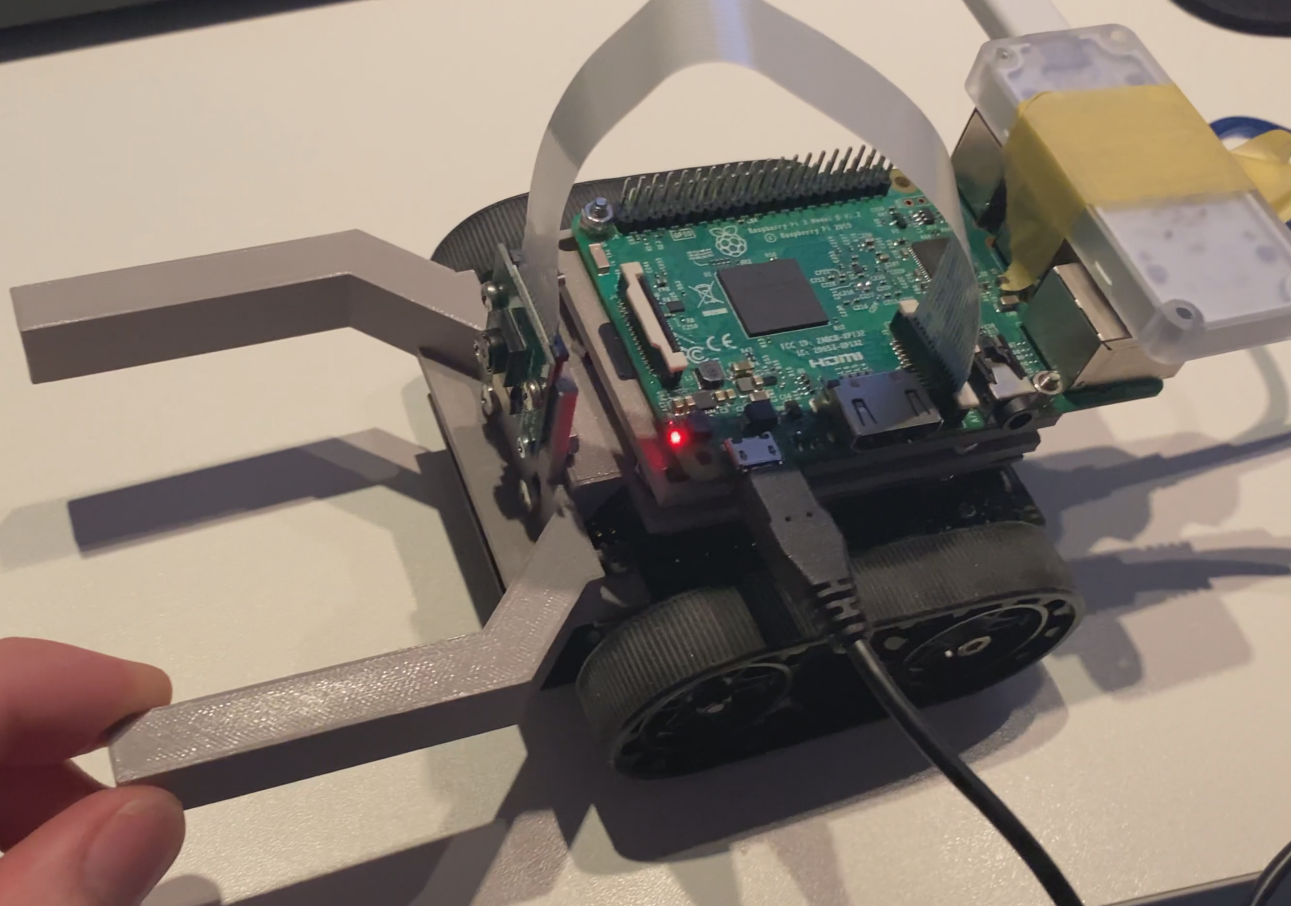
\includegraphics[width=200pt]{img/mount.png}
    \caption{Mount gemonteerd op de Zumo robot}
    \label{fig:mounted_mount}
\end{figure}

\subsubsection*{De webapplicatie}

De web-aplicatie was erg goed gelukt naar onze mening. De app zelf was makkelijk te begrijpen en kwam modern over. Dit komt mede door de singele-page functionaliteit die met React was gemaakt. Het ontwikkelen van de app was ook niet erg lastig en duurde niet erg lang.\\

De integratie met de Python applicatie was ook erg makkelijk met de Flask backend-API. Wel vonden we het jammer dat Flask geen OOP oplossing biedt, aangezien de rest van de applicatie wel zo was geschreven.

\subsection{Wat kon beter}

\subsubsection*{Locatie}

Door niet bij elkaar te zijn, werd de samenwerking op sommige fronten erg gecomprimeerd. Zowel testen als overleggen ging lastiger dan normaal en zorgde voor relatief minder efficiënte werkdagen.

\subsubsection*{BLE}

Het probleem bij onze BLE oplossing was dat de signaal sterkte erg zwak was. Hierdoor ging het signaal vaak op in de ruis. Waardoor de accuratie van RSSI meting erg onbetrouwbaar werd op grotere afstanden. 

\subsubsection*{Stappen motoren}

Omdat er op de Zumo standaard DC motoren zitten hadden wij geen andere keuze dan deze te gebruiken. Helaas konden we deze niet vervangen met bijvoorbeeld stappenmotoren, hierdoor moesten wij voor sommige features van de robot meer ingewikkeldere/minder accurate oplossingen verzinnen. Een voorbeeld hiervan zou bijvoorbeeld zijn hoe vaak we de positie service gebruiken voor kleine veranderingen. In plaats van alleen de positie service gebruiken voor de initiële positie en verder rekenen op de stappen die de motor heeft gezet.

\subsubsection*{Batterijen}

Tijdens het ontwikkelen van de robot konden we geen batterij gebaseerde stroom oplossing bouwen, dit kwam voornamelijk door dat niemand van ons de gereedschap thuis heeft liggen om zo\'n opstelling te bouwen en te testen. Onze uiteindelijke oplossing hiervoor was om de Micro-USB kabel in de Raspberry Pi te laten zitten om als stroomtoevoer te dienen.\\

Helaas zorgde deze oplossing voor een ander groot probleem, namelijk dat de Zumo robot veel moeite had om de kabels waaraan die vast zat mee te bewegen, hierdoor werd het naar rijden erg beïnvloed.

\subsubsection*{Performance}

Tijdens het draaien van het programma merkte we dat de performance een stuk slechter was dan toen alles los van elkaar draaide. Dit komt waarschijnlijk door de hoeveelheid treads die we tegelijkertijd gebruiken. Bij de object detectie merkte we dat we in plaats van 15 FPS nog maar 5 FPS hadden. Dit hebben we uiteindelijk opgelost door de resolutie lager te zetten. Dit zorgt er helaas wel voor dat de detectie minder accuraat en minder ver zal werken.\\

Een manier om dit op te lossen was om de Raspberry Pi 4 te gebruiken. Naast meer ram heeft deze ook twee meer cores. Dit zou de performance van de applicatie goed kunnen bevorderen.

\subsubsection*{Machine learning}

Het installatieproces van Tensorflow was erg omslachtig. Sergi had dit eerst op Linux geprobeerd, maar kwam er later pas achter dat de versie van Tensorflow uit maakte voor het trainproces. Aangezien de Tensorflow versie die we zochten (1.13) niet geinstalleerd kan worden voor Python versie 3.8 moest er worden gedowngrade. Echter is dit erg lastig en niet gewenst op de versie van Linux die gebruikt werd. Er is toen voor gekozen om het trainen op Windows te doen, omdat de tutorial dit ook deed. Naast dat het installatieproces nog omslachtiger was is het uiteindelijk wel gelukt om het model te trainen.\\

Naast de installatie was het trainen ook niet helemaal optimaal. Het trainscript die we gebruikte kon als input alleen maar gelabelde selecties krijgen. Hierdoor konden we geen afbeeldingen zonder labels meegeven. Dit was handig geweest om hard-negatives te trainen zonder ze te labelen. Dit is wenselijk, omdat ze dan niet worden gedetecteerd en alleen onderdeel zijn van het trainingsproces. Nu moeten we de hard-negatives als selectie meegeven, wat er voor zorgt dat ze gedetecteerd zullen worden. Aangezien de hard-negatives erg verschillend waren wordt het detecteren van hard-negatives ook niet altijd goed gedaan. Ook hadden de hard-negatives een witte achtergrond, waardoor dit teveel meegenomen werd in het trainingsproces. In Figuur \ref{fig:detection-positive-negative} is goed te zien hoe erg de achtergrond werd meegenomen in de detectie. Het is duidelijk dat de object detectie nu beter werkt op een achtergrond, wat niet realistisch is. In de toekomst zouden er afbeeldingen moeten worden gebruikt met een achtergrond, of zouden ze zelfs op tennisvelden moeten worden geplaatst. 

\begin{figure}[H]
    \begin{subfigure}{0.5\textwidth}
        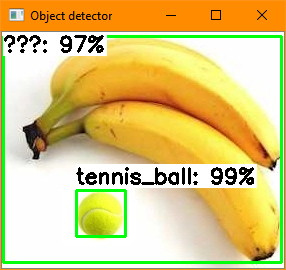
\includegraphics[width=0.9\linewidth]{img/ball_banana_white.png} 
        \caption{Een correcte detectie met een witte achtergrond.}
        \label{fig:ball-banana-white}
    \end{subfigure}
        \begin{subfigure}{0.5\textwidth}
        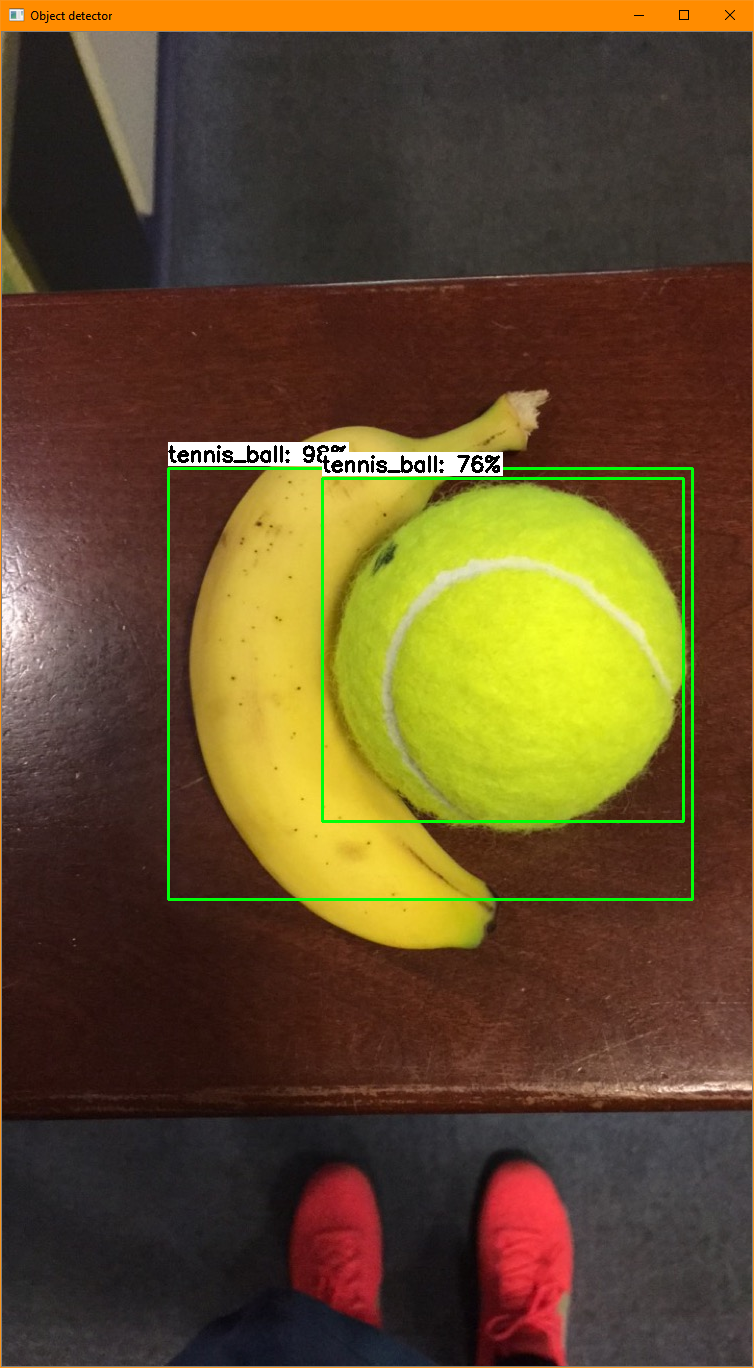
\includegraphics[width=0.5\linewidth]{img/ball_banana_background.png}
        \caption{Foutieve detectie door de realistische achtergrond.}
        \label{fig:ball-banana-background}
    \end{subfigure}
    \caption{Het verschil tussen detectie met een witte- en een realistische achtergrond.}
    \label{fig:detection-positive-negative}
\end{figure}
